\documentclass{article}
\usepackage{amssymb}
\usepackage{amsmath}
\usepackage{graphicx}
\usepackage{adjustbox}
\usepackage{pdflscape}

\graphicspath{{../}}

\title{Progress Report}
\author{Annabelle Cloutier}


\begin{document}
\maketitle

\tableofcontents

\section{ECO-DQN, Max Cut Problem}\label{sec:eco-dqn-explained}

\subsection{Network Structure}\label{sec:network-structure}

All of the below information is based on the work in \cite{eco-dqn}.
The network structure is incredibly generic most of the way through, but notes are written here to avoid having to parse through the equations that describe the network structure in the paper. Note that at any step where learned weights are used, the ReLU function is used on the resulting vector. The only exception is for the last set of learned weights in the readout layer, which instead is a linear output, giving the expected reward for choosing that graph vertex. 

\subsubsection{Node Embedding}\label{sec:node-embedding}

The Message Passing Neural Network (MPNN) structure used converts each vertex into a set of $m$ observations and encodes them into a $n$-dimensional embedding using learned weights. These $m$ observations contain information about the state of the solution with respect to that vertex that they call local observations, as well as global information for the entire candidate solution being considered. The paper states that they use 64 dimensional embeddings and they do in code, but this could be any size. Their code provides parameters for changing the size of these layers through parameters to the network on initialization.

The observations in the paper as well as their justifications for them are as follows: 

\begin{enumerate}
    \item Whether the current vertex belongs to the solution set $S$ or not; 
    
    This is a local observation. The reason they state this observation is important is that it provides useful information for the agent to make a decision on whether the vertex should be added or removed from the solution set. 

    \item The immediate cut change if the current vertex state is changed;
    
    This is also a local observation. Just as with the above observation, they state this provides useful information for decision making. They also state is that it allows the agent to exploit having reversible actions. This makes intuitive sense, as knowing the difference between having a vertex in the solution or not can allow the agent to learn to make an informed decision on whether to add or remove it, or in this agent's case, possibly reversing an action, based on the change of the cut value if they were to change that vertex' state.

    Not mentioned in the paper is that this result is normalized by the largest non-zero change in the cut value from the empty solution set. Intuitively, this is the largest non-zero weight of a vertex, being the sum of the weights connected to the vertex. This does not guarantee that all values will be normalized between $-1$ and $1$, but it does give a frame of reference to know how much better a greedy action would be in the current candidate solution compared to an empty solution set. 

    \item The number of steps since the current vertex state was changed;
    
    Also a local observation. For this observation, they mention that it provides a simple history to the agent to prevent looping decisions. They also state it allows the agent to exploit reversible actions just as with observation 2. Therefore, this specific observation could be important as the value increases as the vertex remains unchanged, which can entice the agent to choose vertices that have not been chosen in a long time to encourage exploration, as well as discouraging it from getting stuck in a local minimum, changing the same vertices repeatedly over the decision making stage.

    This result is normalized by the total number of steps in an episode (which I'll define later), to range each value between $0$ and $1$. 
    
    \item The difference of the current cut value from the best observed;
    
    This and all future observations are global. This observation they state ensures the rewards are Markovian. Just as with observations 2-4, this observation they also mention allows the agent to exploit having reversible actions, which makes intuitive sense. The agent knowing the difference between the current cut value and the best one observed, along with the other observations, can allow the network to make informed decisions on whether the current solution is a promising set to explore.

    The way this is calculated is by comparing the current cut value to the best observed. Not mentioned in the paper is that they use the absolute value, but because the best observed is always chosen prior to a decision being made, this value is necessarily always either $0$ (the current candidate is the best observed) or larger, as the best observed is necessarily a larger value cut for the maximum cut. This detail is important  This value is also normalized by the largest non-zero weight of a vertex. 

    \item The distance of the current solution set from the best observed;
    
    This observation as with observation 5 they state ensures the rewards are Markovian. Again, this observation allows the agent to exploit reversible actions. 

    The difference between this and observation 5 is that observation 5 compares the cut value only. This observation compares the solution sets and counts the number of vertices that differ between the best observed solution set of vertices and the current one. This is not explained in the paper, but can be seen in the code.

    Example for clarity:

    Best observed bitmask of vertices: $[0, 0, 1, 0, 1]$

    Current bitmask of vertices: $[0, 1, 1, 0, 1]$.

    Distance = 1. 

    \item The number of available actions that immediately increase the cut value;
    
    Once again, this observation ensures Markovian rewards, they also mention that this allows exploitation of reversible actions, which is more easily understandable. Although this information can technically be inferred through observation 1, that information may not be transmitted throughout the entire graph in a finite number of steps in the message passing stage of the neural network. 

    \item The number of steps remaining in the episode
    
    The only reasoning they have for this observation is that it accounts for the finite time used for solution exploration. This information can allow the network to make different decisions based on how deep in it is exploration it is. The exact behaviour isn't necessarily predicted, but their findings do show that the further in an episode the network reaches, the more likely it is to revisit a vertex. 

\end{enumerate}

\subsubsection{Edge Embedding}\label{sec:edge-embedding}

The edges for each vertex are also encoded into a separate $n$-dimensional embedding, same size as for each vertex, once again learned. The input for this step is the set of $m$ observations of the neighboring vertices catenated with the weight on the connecting edge, creating an $m + 1$ dimensional vector for each neighboring vertex. All of these vectors are then summed item-wise and passed through a learned layer, creating an $n - 1$ dimensional vector. At this stage, the resulting $n - 1$ dimensional vector is divided by the number of neighbors and catenated with the number of neighbors, resulting in an $n$ dimensional vector, and passed through another learned layer, resulting in an $n$-dimensional embedding representing the information about the neighboring vertices and the edges connecting them.

The end result of these two steps are an $n$-dimensional embedding representing a vertex and another representing it is neighbors, all created using the same learned weights for every vertex. In the paper, $n$ is chosen as 64, but this value could be anything in theory, which would just enlarge the size of the network. The exact reason behind this decision is not mentioned and seems arbitrary. However, the optimal size of a neural network could likely be found experimentally through training multiple networks of different sizes. It's likely that the authors believed that a 64 dimentional embedding of the 7 observations was enough to contain the information relevant to the problem to get a good performance, and their results seem to show that this hypothesis was at least partially correct. One very likely decision for this reason is to ensure that all of the network layers had memory sizes in powers of two as this could improve performance at the hardware level on the GPU \cite{cuda-practices}.

\subsubsection{Message Passing}\label{sec:message-passing}

Here there is a message pass layer and an update layer. The message pass for a vertex multiplies every neighbouring vertex's node embedding by the weight on the connecting edges and takes a sum over all of these neighbouring vertices. It then normalizes by the number of neighbours and catenates the edge embedding for the current vertex. This resulting vector is of size $2n$, an embedded vector representing the neighours for that vertex. This vector is passed through a set of learned weights, resulting in a $n$-dimensional vector. 

The next is the update layer, which is the embedding for that vertex, catenated with the message, resulting in a vector of size $2n$. This is once again passed through another set of learned weights, into an $n$-dimensional vector, representing the new node embedding for that vertex. This new embedding can then be used to perform another pass of message passing and updating.

The message then update process is performed $K$ times. Mentioned in the paper and corroborated in the code, this is done 3 times, but can be done however many times necessary, just as the network size can also change.

\subsubsection{Readout}\label{sec:readout-layer}

The readout layer goes through each vertex, summing the node embeddings for the neighbors of that vertex, dividing the result by the number of vertices in the entire graph and then passing it through learned weights, resulting in an $n$-dimensional vector.

The embedding for the vertex itself is then catenated to it, resulting in a vector of size $2n$ which is passed through another set of learned weights (without applying ReLU), giving in a single output value. Because this message passing process and readout is performed on very vertex, this gives you $|V|$ Q-values. The maximum Q value, which is associated to a particular vertex, is used to determine which vertex will have an action performed on it. Because there is only one Q value per vertex, this is associated to one single action that can be done on any vertex, which is to either add or remove it from the solution. For the maximum cut, which they use as an example in the paper, this is analogous to moving a vertex between the left and right sides of the cut depending on it is current state. 

\subsection{Rewards and Training}\label{sec:rewards-training-eco}

\subsubsection{Q Function and Q values}\label{sec:q-function}

The Q function is an idea derived from Q-learning \cite{qlearning} which proposes a way for an agent to learn how to behave in an environment. It is defined as the expected value of the discounted sum of future rewards for any state-action pair of an environment. When an optimal Q function is derived, the agent chooses which action to perform in a certain state by selecting the state-action pair which corresponds to the largest Q-value, which is expected to give them to largest reward. The equation following equation represents this idea:
 
$Q^\pi(s, a) = E[\sum_{t=0}^{\infty} \gamma^t R(s_t) | s_0 = s, a_0 = a, \pi]$

where $\pi$ is a policy, mapping a state to a probability distribution over the actions, $R(s)$ is the reward for a given state and $\gamma^t$ is a discount given to change whether the agent prefers immediate or future rewards.

This Q function is learned by a Markov decision process. The agent traverses the environment and rewards are given at each step depending on the result of the action the agent performs.

Trying to find this Q function was known to be unstable or even diverge when nonlinear function approximators, like neural networks, were used to try and represent it \cite{td-func-approx}. In \textit{Mnih et al.}, they propose an approach to Q learning with two main ideas; namely experience replay and an iterative update, adjusting the Q values towards target values only periodically, while progressively constructing a training set throughout training, ensuring that the agent not only explores the environment, but also that the neural network can stabilize by forcing it to review previous state-action pairs \cite{deepmind_2015}. The agent during training only chooses the actions associated with its current policy with probability $\epsilon$ and otherwise chooses a random action. They demonstrate experimentally that with these ideas, they were able to train a model that had significant performance improvements compared to other existing models on 49 different Atari games.

These ideas are replicated in the training of ECO-DQN. For every episode in the training phase, a random graph is sampled with a random solution set. Then, for each time step in that episode, which they set to $2|V|$, the agent chooses a random vertex based on the existing Q function with a probability $\epsilon$ and a vertex dictated by it is Q function otherwise. Then, the starting state, chosen vertex, reward and resulting state are added to the experience replay memory. Finally, after some fixed set of episodes, the network is updated by stochastic gradient descent on a minibatch sampled from the experience replay memory.

They set $\epsilon = 1$ and decrease it linearly to $\epsilon=0.05$ over the first $10\%$ of training. 

\subsubsection{Reward Shaping}\label{sec:reward-shaping-eco}

The reward in a certain state is given by the difference between the cut value in that state and the highest cut value seen so far in the episode, divided by the number of vertices. If the difference is negative, it is instead set to 0, meaning the current state is worse than the best one seen. The justification behind this choice is that a negative reward will discourage the agent from exploring states that give an immediately worse cut value, even if other cuts including that change later on may give better cut values overall. If this were to happen, it could discourage the agent from exploring different cuts and possibly cause it to stay stuck in a very small space near a local optimum. Because previously seen optimal states are stored in memory and returned as the result, it is therefore beneficial to later let the agent explore more states in an attempt to find more locally optimal states, even if not always better than the previously seen local optimum.

They also define a reward for reaching previously unseen locally optimal states of $\frac{1}{|V|}$. This is once again to encourage exploration. They state that local optima in combinatorial problems are typically close to each other and therefore by giving rewards for reaching new local optimums, the agent learns to hop between them during training as it is rewarded for this behaviour. In being rewarded for finding more unseen local optimums while being near a global optimum, it increases a behaviour pattern that has a propensity to finding this global optimum. Without this, they state that because there are far too many states to be visited in a finite time, which is typical for combinatorial optimization problems, it is therefore useful to focus on these subsets of states near local optimums.

There is no exact reason stated for the choice of value, however it can be hypothesized that if a constant value is chosen, this could cause disproportionate reward shaping on different sized graphs. For example, graphs that have significantly more locally optimal cuts could end up rewarding the network too much for simply finding local optimums instead of attempting to find a global optimum, while using the exploration of local optimums as a means to that end. Because larger graphs are likely to have more locally optimal states, it therefore makes sense to choose a value that decays as the size of the graph increases. Therefore a reward proportional to the inverse of the number of vertices in the graph makes the most sense. 

The choice to not randomly change states when a new local optimum is found appears to be mostly a choice that the authors made intentionally as they want the network to find some space that has numerous locally optimum states near each other to explore, and the best way to do this is to encourage finding nearby local optimums instead of sending the agent in different random directions every time a new local optimum is found. They do state that because there are far more states than can be visited within a finite time period, it is therefore more useful to find some local optimums that are near each other and explore that specific space of possible solutions.

They demonstrate this behaviour by observing the probability during any given timestep that the agent will either revisit a state, find a locally optimal state or find the maximum cut on the validation set. They show that as the number of timesteps goes up, the probability that the agent revisits a state goes up, as does the probability of finding the maximum cut, while the probability that the agent finds a local optimum goes up very quickly and stabilizes for the rest of the time steps, showing that the agent picks a certain set of states and explores the space around them to find new local optimums by revisiting previously seen states. This also demonstrates that the agent does not tend to get stuck in a specific local optimum and refuse to explore. 

One thing this paper does not tackle is the issue of invalid solution states and how this would affect reward shaping, especially in a situation where the agent would be allowed to revert previously made actions. This isn't necessary for the Maximum Cut Problem, as any partition of the graph into two containing all vertices is a valid cut, but problems like the Traveling Salesman, Minimum Vertex Cover, Minimum Bisection and problems like the Knapsack Problem that are not graph problems could possibly include states that are not valid solutions by either not being a complete path, not covering every edge in the graph, having two sets of different sizes or having an overfull bag, respectively for each problem. This becomes an issue for reward shaping especially, as it would therefore become impossible to compare invalid states to valid ones. A possible solution for this issue is to disallow invalid solutions, but with a problem like the Minimum Bisection, any change made to a valid state immediately makes it an invalid candidate solution. Because of this, some framework to allow an agent to explore invalid candidate solution states should be devised. 

\subsection{Discussion on Generalization}\label{sec:discussion-generalization-eco}

The internal structure of the MPNN should be generic for any graph or problem as it merely propagates information about observations on vertices throughout the graph. However, because of the large number of changes that would likely need to be made to observations (inputs) as well as the interpretation of the output for many other types of problems, it is likely that some changes to the internal structure would have to be made for the agent to make more educated decisions on new problems. 

The main issue comes with the output and it is interpretation. Each vertex is represented by a single value as the output, and that value is interpreted as adding or removing it from the solution set, in the context where the solution is a subset of the vertices in the graph. More specifically for the Max Cut problem, the vertex associated with the maximum Q-value (output value) is taken and then either added or removed from the solution set, depending on whether it already belongs to it or not. This approach works fine for a problem like Maximum Cut or Minimum Vertex Cover where the solution can be represented as a set representing chosen vertices for the solution, however any extra constraints forces the output interpretation to be completely redesigned. 

For example, the Traveling Salesman Problem where the solution is an ordered list of vertices could pose issues as the current implementation of simply adding or removing a vertex from the solution may not be adequate to allow the network to explore different states, and may have to be redesigned, like not allowing the network to remove states that aren't at the tail of the current path or outside of the current path. Any other problem where the solution is an ordered list of the input would have this same issue.

The Minimum K-Cut Problem which can have an arbitrary number partitions of the graph would also not work with the current model as it would require extra decision making on deciding which set to move a vertex to. Because the number of sets can also change, this means the size of the output would have to change as the solution changes which would mean a new network would have to be trained for every graph size or k-value for the cut, or some significant rework of the output interpretation would have to be made. Any other problem where the solution is to split the input into $k$ sets would have this same issue.

To verify whether this network structure is truly generic, we can try the exact neural network structure on a few different problems by modifying the observations and rewards specifically for those problems. We can do this trivially for the Minimum Cut, and some work will be done to test this on the Minimum Vertex Cover, a problem tackled in the paper for S2V-DQN which is not discussed or evaluated in the ECO-DQN paper.

\subsection{Benchmarks}\label{sec:benchmarks-eco}

The paper displays the performance of the network in reference to S2V-DQN, a similar paper where the algorithm does not allow for reversing actions \cite{s2v-dqn}. They also compare its performance against modifications of itself, namely where some observations are restricted, intermediate rewards are not given for reaching locally optimal solutions, as well as stopping it from reversing its actions. 

They also a MaxCutApprox algorithm, which is a greedy algorithm choosing the vertex that provides the greatest cut improvment for one full episode of $2|V|$ steps. They implement two variations of this, one where it can reverse actions and one where it cannot reverse it's actions. 

They also use an approximation ratio $C(S^*)/C(S_{opt})$. However, because $S_{opt}$ cannot be calculated exactly, they use multiple optimizations. Specifically, they use CPLEX, an integer programming solver, as well as a pair of simulated annealing heuristics by Tiunov \textit{et al.} (2019) and Leleu \textit{et al.} (2019) in order to calculate $S_{opt}$. 

The implementation of these different algorithms is not included in the codebase provided. However, the optimal solutions and cut values for the ER graphs with 40 vertices are provided for the testing graphs. The validation graphs of all sizes have their maximum cut values included.

They use GSet graphs G1-10 and G22-32 as well as the Physics/Ising dataset as benchmark graphs. These, as well as their optimal cuts and solutions are provided in the codebase. 

\subsection{Graph Generation}\label{sec:eco-graph-gen}

They train and test on Erdos-Renyi \cite{erdos} and Barabasi-Albert \cite{albert} graphs. For training, they generate random graphs and perform a full episode of solving them, adding each state, action and reward to the experience replay memory. For testing, they have a set of 50 graphs, being either ER or BA graphs with different numbers of vertices which are used to compare the trained network to other algorithms. 

\section{Code}\label{sec:eco-code}

The code includes most, but not all, of the tests ran in the paper. Some of the algorithms are not included as well.

\subsection{Running Code}\label{sec:eco-running}

They very generously provide a README file that specifies the exact commands to run in order to train, test and validate networks. These simply run specific files, namely the test\_eco.py and train\_eco.py files, for the respective graph sizes, so they can also be run by doing the typical process for running a python file. However, there is no code for reproducing the specific tables and plots. The data saved that is capable of generating the tables and plots in the paper are saved and therefore could be used to generate them. The code for generating that data is also provided and can therefore be analyzed and used for different problems, as different algorithms would have to be used for comparison.

\subsection{Graph Implementation}\label{sec:graph-implementation}

The random graphs for training are generated using the NetworkX library which includes the implementation for random ER and BA graphs. For training, they use the classes defined in src/envs/utils to generate new graphs at each step, adding every action done on the new graphs to the experience replay memory which is used to train the network. This ensures every training session is random and includes different data. The testing graphs are all the same, but change depending on the size of the training networks. For example, a network trained on graphs with 40 vertices will also have it is performance tested on graphs with 40 vertices. This behaviour can be modified to verify whether a network trained on large graphs still performs well on smaller graphs as well as larger ones by making modifications to the code.

\section{Minimum Cut}\label{sec:min-cut}

\subsection{Reward and Observations}\label{sec:reward-shaping-min-cut}

The Minimum Cut is still combinatorial optimization problem that could be solved by ECO-DQN as the problem structure is identical to the Maximum Cut but instead minimizes the cut. To confirm that the idea is expandable to other problems, we will train an identical structure, using the negative of the cut value for determining the solution's reward with respect to the best observed, forcing the network to minimize the cut instead of maximize it as it will now receive greater rewards for smaller cuts. 

$R(S) = max(0, -C(S) - -C(S^*))$. 

We can use identical observations as defined in , as these problems do not differ in any way other than how the measure of the quality of a solution is evaluated.

Just as with the original idea for ECO-DQN, at each step the best found solution is simply the solution with the minimal cut found so far during an episode. This best seen is then returned at the end of the episode after $2|V|$ steps.

\subsection{Results}\label{sec:results-min-cut}

The result of training found in %Figure \ref{fig:min-cut-training} show this network is very similar to the maximum cut found in the ECO-DQN paper. It starts giving random solutions and eventually reaches a point where the cut value found stabilizes on the test graphs. This demonstrates that the network structure can be utilized to solve other problems. This was not tested against other algorithms, so it is possible that the cuts found are not minimal, but this provides some indication that at least the network can learn something about other problems than the Maximum Cut Problem. 


\section{Minimum Vertex Cover}\label{sec:mvc}

A vertex cover is a set of vertices such that every edge in a graph has at least one endpoint in the that set of vertices. More formally, given a graph $G = (V, E)$, provide a vertex cover of $G$, being $V' \subset V$, such that for each edge $(u, v) \in E$, at least one of $(u, v)$ belongs to $V'$. We want to find the smallest cardinality of any $V'$. This smallest vertex cover $|S|$ for a graph is known as the Minimum Vertex Cover. Finding this cover is known to be NP-hard. To tackle this issue with the approach in ECO-DQN, a few problems need to be solved.

First, because this is not a cut problem, different observations that do not rely on calculating a cut need to be devised that can adequately report on the information about the vertices in the solution as well as the current candidate solution as a whole. 

Further, some of the candidate solutions for this problem can be invalid candidate solutions. Due to this fact, the current reward system needs to be modified to take this into account, as we can no longer simply calculate the difference between the return values (i.e. $|V'|$) as some $|V'|$ that the network can generate may not be valid vertex covers. Some punishment needs to be made for these invalid candidates, and a reward needs to be devised for finding smaller vertex covers. For this problem specifically, you can in theory disallow invalid candidates from being searched to avoid this issue. However, for the sake of allowing generality to other problems where this may not be the case such as the Minimum Bisection, we will still allow invalid candidates to be searched. 

Thankfully, some of these are somewhat trivial to solve, like the observations and reward, by either using ideas from ECO-DQN \cite{eco-dqn} and the similar S2V-DQN \cite{s2v-dqn} which does not allow for exploration/undoing actions but does tackle the Minimum Vertex Cover.

\subsection{Observations}\label{sec:observations-mvc}

In ECO-DQN, they have their set of observations from which we can draw to design the observations for the Minimum Vertex Cover. Some of these are even somewhat trivial to convert, namely:

\begin{itemize}
    \item Observation 1, "Vertex sate, i.e. if $v$ is currently in the solution set, $S$" is very easily translatable. We can directly copy this information, irrespective of if the current state is a valid solution.
    \item Observation 3 "Steps since the vertex state was last changed". This one also can be directly copied.
    \item Observation 4 "Difference of current cut-value from best observed". We will translate this to the difference between the current cover set size and the best cover set size. we will ignore the validity of the solution, so as to adquately represent all of the information about the current candidate without hiding some of the information due to a candidate solution being invalid.
    \item Observation 5 "Distance of current solution set from the best observed". In the paper they do not define this, but it is explained through their implementation in Section \ref{sec:node-embedding}. We can also use this information for the Minimum Vertex Cover in the same way.
    \item Observation 6 "Number of available actions that immediately increase the cut value" can also be translated. Namely, counting the number of actions (or vertices) that when flipped will reduce the number of vertices in the cover. Again, in this case we will ignore the validity of the solution created by changing that vertex state.
    \item Observation 7 "Steps remaining in the episode". This, once again, can be directly copied.
\end{itemize}

Observation 2 in the ECO-DQN paper was the immediate cut change if the vertex state is changed. We would interpret this as the immediate change in the size of the vertex cover's set ignoring validity, but this is implied by Observation 1 for the Minimum Vertex Cover and would therefore provide no added information to the network. This observation can therefore be discarded.

With all of this done, we want to add information about the change in validity of the candidate solution both for local vertex changes, as well as compared to the best seen solution. Therefore, we can add the following observations:

\begin{enumerate}
    \item Immediate change in the number of edges covered on vertex flip. This counts the number of edges that were previously uncovered but are now covered as a negative number and positive if it increases the number of edges that are uncovered. This value is normalized by the total number of edges in the graph to account for graphs with different numbers of edges and vertex degrees.
    \item The solution's validity on vertex flip. This represents whether the solution produced by changing whether the vertex is in $V'$ or not is valid ($1$) or invalid ($0$). 
    \item Number of actions that immediately increases the number of edges covered by the solution. This simply counts the number of actions that make the solution approach validity. This value is normalized by the number of vertices in the graph.
    \item Difference in number of edges covered from current solution and best observed. This counts the number of edges covered by the best observed solution and the current candidate and compares the values. This value is positive if the current candidate covers less edges than the best observed. This value is normalized by the number of edges in the graph.
    \item Validity of current solution. 
\end{enumerate}

This means we have the following observations for the Minimum Vertex Cover:

\begin{enumerate}
    \item Observation 1: Vertex state
    \item Observation 2: Steps since the vertex was changed 
    \item Observation 3: Immediate change in the number of edges covered on vertex flip 
    \item Observation 4: Immediate change in the solution's validity on vertex flip 
    \item Observation 5: Difference of current set size from best observed 
    \item Observation 6: Difference of number of edges covered by current solution from best observed 
    \item Observation 7: Distance of current set from best observed 
    \item Observation 8: Number of actions that immediately reduce the set size
    \item Observation 9: Number of actions that immediately increase the number of edges covered by the solution 
    \item Observation 10: Validity of current solution 
    \item Observation 11: Steps remaining in episode 
\end{enumerate}

This leaves us with local observations 1-4 and global observations 5-11 which all grant information about the state of the solution at that time, both for local changes and global differences from the best observed solution.

\subsection{Reward Shaping}\label{sec:reward-shaping-mvc}

Due to the difference between how proposed solutions are going to be in the Maximum Cut and Minimum Vertex Cover, some different rewards are going to be required to adequately represent the problem. In ECO-DQN \cite{eco-dqn}, the reward for a certain state is framed as

$R(S) = \frac{max(0, C(S) - C(S^*))}{|V|}$

where $C(S)$ is the cut value for state $S$ and $S^*$ will be the previously best seen cut value. They also grant intermediate rewards $\frac{1}{|V|}$ any time a new locally optimal cut is found, which is a cut that has not yet been seen where any change to a vertex reduces the value of the cut.

In S2V-DQN \cite{s2v-dqn}, the reward for a Minimum Vertex Cover they define as $R(S, v) = -|S| - -|S'|$ being the change in their cost function when going from state $S$ and adding vertex $v$ to it, resulting in state $S'$. In these cases, the state is the set of vertices chosen for a candidate solution. We can reformulate their idea slightly to coincide with the idea in ECO-DQN to allow for exploration by instead looking only at defining the reward on a specific state in comparison to the best seen instead of the previous state.

In our case, the best seen is not so simply defined. Because constructed candidates may not be valid, some way to compare invalid candidates to valid ones has to be devised such that we can choose a previous "best" candidate to use as a comparison for future candidates. What we want is a reward mechanism that allows valid candidates to always be chosen as the best over invalid ones, as well as for valid candidates to be compared to each other in such a way that a candidate that improves the solution gives a better reward than ones that don't. Similarly for invalid candidates, we would like for them to be compared to each other in such a way that an invalid candidate that is closer in some measure to being a valid solution gives a better reward than one that is further away. One way to do this is to ensure that valid solutions gives positive rewards increasing in magnitude depending on it is quality, and for invalid solutions to give negative rewards increasing in magnitude depending on it is relative lack of closeness to being a valid candidate.

For the Minimum Vertex Cover, the score of a valid candidate can be defined in a similar way as in S2V-DQN by calculating the size of the set not including the current candidate solution, $|V - S|$. This grants higher scores to smaller candidate set sizes. Therefore, when comparing valid candidates using the same reward function as ECO-DQN, we will get positive rewards for smaller set sizes. We can of course normalize this value by the number of vertices to accommodate different graph sizes. In order to account for invalid candidates being scored more highly in this measure, we'll multiply this value by $0$ if the candidate is invalid and $1$ otherwise. This function we can simply call the validity of $S$.

For invalid candidates, their scores can be the negative of the number of edges not covered by the candidate. Therefore, invalid candidates being compared will give greater positive rewards for getting closer to a valid solution. Of course, this also will result in positive rewards for moving from an invalid candidate to a valid one. To normalize this, we can use the number of edges in the graph, to account for graphs with differing numbers of edges. A property of using this for getting the score of an invalid candidate is that valid candidates always have exactly zero uncovered edges.

Including these two ideas, we can define the score of a candidate for the Minimum Vertex Cover as being 

$score(S) = validity(S) * |V - S| - edges\_uncovered(S)$. 

Where $S$ is the current candidate solution state being evaluated. Normalizing this score would be similar,

$norm\_score(S) = \frac{validity(S) * |V - S|}{|V|} - \frac{edges\_uncovered(S)}{|E|}$. 

To elaborate on the previous point mentioned in the Observations section of the Minimum Vertex Cover, this means that when starting from the empty candidate solution, the largest possible change in score would be difference between the score for $|V - S| = |V|$ and the score for an invalid solution, maximizing the number of edges uncovered such that when a vertex is added, the solution is now valid. This would be like adding the vertex of highest degree to the current candidate, resulting in the empty solution, while also being a valid solution. 

When calculating the reward, we can use the same idea as ECO-DQN, $R(S) = max(0, norm\_score(S) - norm\_score(S^*))$, where $S^*$ is the previously best seen candidate. Of course, by comparing scores we can select the best score as the best previous candidate, as the scores increase in value for valid candidates of smaller set size and decrease as the set size becomes larger or as the candidate is not valid. The following shows the results of comparing the scores of different solutions $S$ and $S^*$ for determining a new best seen candidate:

\begin{enumerate}
    \item Invalid $S$ compared to invalid $S^*$ only give positive rewards when $S$ is closer to being valid than $S^*$. Therefore $S$ is only a better candidate if it covers more edges.
    \item Invalid $S$ compared to valid $S^*$ will never give a positive reward. Therefore an invalid $S$ cannot become the new best seen if $S^*$ is a valid candidate. This ensures we always return a valid candidate (if one is found) at the end of a search.
    \item Valid $S$ compared to invalid $S^*$ will always give a positive reward. Therefore is $S^*$ is invalid and $S$ is valid, $S$ becomes the new best seen candidate.
    \item Valid $S$ compared to valid $S^*$ will only give positive rewards if $S$ is a better solution than $S^*$. Therefore $S$ becomes the new best seen only if $|S| > |S^*|$.
\end{enumerate}

As with ECO-DQN, we will also give intermediate rewards for finding new local optimums in order to avoid situations where rewards become incredibly scarce and to encourage it to find new locally optimal states to explore. This reward will be the same amount as well, of $\frac{1}{|V|}$ to account for larger graphs having more locally optimal states.

\subsection{Training}\label{sec:training-mvc}

Training this network will be algorithmically identical to ECO-DQN \cite{eco-dqn} using the ideas from Deep Q-Learning described in \textit{Mnih et al.} \cite{deepmind_2015}.

Because the original test graphs were generated using discrete edges weights of either $1$ or $-1$, we first recreate the test graphs with the same edges but setting all the weights to $1$. This functions as an undirected, unweighted graph for evaluating a Minimum Vertex Cover. All of the training graphs will also be generated using uniform weights, on ER graphs with edge probability of $0.15$. Training and testing graphs will have the same number of vertices.

Within these parameters for training and testing graphs with $|V| = 20$, the network seems to rapidly improve it is performance on the test graphs and reaching a plateau where it remains for the remainder of the training time. This same trend is observed for larger training graphs. % Figures \ref{fig:training-mvc-20} and \ref{fig:training-mvc-60} show the training loss and average solution found on the testing graphs over the training period.


\subsection{Testing}\label{sec:testing-mvc}

To test the network, it was compared to other algorithms on a set of validation graphs of different sizes. First, the CPLEX linear program solver was set to solve the Minimum Vertex Cover. I also used a greedy algorithm which takes an initial state $S \subseteq V$ and makes greedy actions for $2|V|$ steps based on the score function defined for the neural network. I also implemented a matching algorithm, which selects a random uncovered edge and puts the nodes incident on the edges into $S$. Once there are no more uncovered edges, the algorithm terminates. I also evaluated the minimum weighted cover implemented by Python's NetworkX library, which is based on the work of \textit{Bar-Yehuda and Even} \cite{min-weighted-cover-bar}, that has a worst case run-time of $O(|E| * log(|V|))$ and approximation ratio $2 - \frac{1}{k}$, where $k$ is the smallest integer that satisfies $(2k - 1)^k \ge |V|$. 

Because some of these algorithms are randomized either through implementation or input, any of these were instead run 50 times on each validation graph and the mean solution was selected as the found solution for that graph. The following results show the average cover found by CPLEX, matching algorithm, greedy algorithm with a randomized initalization and empty initialization, local-ratio algorithm and three initializations for the neural network; one where the initial states were random in which case the mean solution found was used over 50 attempts from random states, one test from an empty starting state, and one test from the state where every node is in the cover. Figure \ref{fig:test-20} includes the results found for training the network on graphs with $|V| = 20$.

These results show that the Minimum Vertex Cover is likely a relatively easy problem to solve on small graphs, as the network gets very close to the optimal solution on average, but only marginally improves on the solutions found by the minimum weighted cover solution from \cite{min-weighted-cover-bar}, as well as the greedy solution, which picks greedy for edges and culls vertices randomly until a local optimum is found or the algorithm terminates. More tests on graphs significantly larger than the current ones evaluated should be run to determine whether this truly scales up to large graphs or the performance degrades.

\section{Generalization, Single Subset}\label{sec:generalization-single-subset}

In order for this network to solve different problems, the observations, rewards and actions needs to be modified in such a way that they can be generalized to other problems on graphs with an input $G = (V, E)$. Currently, the most intuitive of these to generalize is the actions. In the network's current state, the action is defined in a way that exclusively works for problems where the solution is a subset $V$, minimizing or maximizing some function. For example, in both maximum and minimum cut problems, the solution is a subset of the vertices of a graph. For the Minimum Vertex Cover, this principle also applies, as the solution will be some $S \subseteq V$. This specific type of output representation exists for numerous graph problems. For example, the Minimum Quotient Cut also requires the solution to be a subset of $V$. Therefore, if some way of measuring a reward and observations for this problem exists, it should also be solvable with this network structure. In general, due to the way the actions are defined through the Q function, any problem where the solution is some $S \subseteq V$ should be a target of study for this network to be able to solve. 

\subsection{Reward}\label{sec:reward-generalized}

Based on the results we've achieved in the Minimum Vertex Cover, the idea that a measure for the solution's quality subtracted by a measure for invalidity is a good place from which to start generalizing. A simple way to do this is to define a function that gives a positive score based on the measure of a candidate state as defined by the problem statement. Determining this function differs between maximization and minimization problems as the value of the reward will change in magnitude based on the measure. For invalid candidates, we'll need to create some measure to evaluate the distance from a valid candidate. This value can then be increasingly large based on the distance and only gives a value if the problem is invalid. This is entirely problem dependent and therefore needs to be considered differently for every problem. One specific restriction on this invalidity is that if the invalidity measure can only be determined by solving some other NP problem, then there will be no way of correctly evaluating the invalidity. This is important for a problem like the Maximum K-Colourable Induced Subgraph problem. However, there are three generally applicable ideas for some problems:

\begin{enumerate}
    \item Problems that determine validity based on a count of vertices can have their validity measured by the number of vertices that need to be removed from $S$ and into $V - S$ in order to be valid.
    \item Problems that determine validity based on a count of edges can have their validity measured by the number of edges over or under the problem requirement that would be necessary to make the current candidate valid. 
    \item Problems that determine validity based on a constraint being satisfied by some function of the candidate solution can have their validity determined by the difference between the current candidate's value based on that function and the requirement. For example, in the Maximum Edge Subgraph problem, $|S|$ must equal a positive integer $k$. We can therefore compute an absolute difference between $|S|$ and $k$ to determine a reward for invalidity.
\end{enumerate}

With all of this in mind, we'll have a general idea of a function for the score $score(S)$ of a candidate solution being the invalidity measure, which I'll refer to as $invalidity(S)$, subtracted from the problem measure score, which I'll refer to as $measure\_score(S)$. To combine these, we'll need the function for validity of $S$ that we defined in Section \ref{sec:reward-shaping-mvc}, which we'll refer to as $validity(S)$. Combining these we'll get:

$score(S) = validity(S) * measure\_score(S) - invalidity(S)$

To normalize this score to be used in the reward function, we can use an upper bound for the problem measure score $UM$ and an upper bound for the invalidity measure $UI$ to guarantee the score for a solution being in the interval $[-1, 1]$. 

$norm\_score(S) = \frac{validity(S) * measure\_score(S)}{UM} - \frac{invalidity(S)}{UI}$

In the end, repeating what we did with the Minimum Vertex Cover from the idea in ECO-DQN, we can then define the reward for a candidate solution as 

$R(S) = max(0, norm\_score(S) - norm\_score(S^*))$

This echoes exactly our mechanism for the Minimum Vertex Cover, where $measure\_score(S) = |V - S|$, $invalidity(S) = edges\_uncovered(S)$, $UM = |V|$ and $UI = |E|$.

\subsubsection{Maximization Problems}\label{sec:generalized-max}

We can easily define the score of a candidate solution for a maximization problem by defining it exactly by the measure. For any problem where this measure can be a negative value, we can find a negative lower bound for the solution measure and offset every reward by this value to make them positive. This lower bound for the measure can be defined as $abs(min(0, LB))$, where $LB$ is the actual lower bound for the measure. In this way, we can define $measure\_score(S) = measure(S) + abs(min(0, LB))$. In this case, we can also define the value for $UM = UB + abs(min(0, LB))$, where $UB$ is an estimated upper bound for the measure.  

\subsubsection{Minimization Problems}\label{sec:generalized-min}

For minimization problems, we'll instead need to define the measure score by using values that invert the order of the measure scores for different candidates. The simplest way to do this is exactly as was done in the implementation of the Minimum Cut problem where we change the score to be the negative of the measure. However, this will result in negative scores and as such, negative rewards. To make all of these values positive, we can simply add the positive upper bound of the measure to every score to guarantee that the value will be positive. Therefore, $measure\_score(S) = - measure(S) + max(0, UB)$. If every single measure is negative, this therefore guarantees only positive scores for valid candidates to a minimization problem. We also need to define a new $UM$ for minimization problems. In this case, $UM = - LB + max(0, UB)$ uses the negative of the theoretical lower bound of the measure and offsets it by a positive upper bound to the solution to guarantee all values for the measure's score are normalized to the range $[0, 1]$. Based on our Minimum Vertex Cover implementation, this would be $- |S| + |V|$ or $|V - S|$ for the $measure\_score(S)$. The value for $UM$ would therefore be $|V|$ as the lower bound for the Minimum Vertex Cover is $0$. This is precisely the mechanism used previously.

\subsection{Observations}\label{sec:observations-generalized}

In Section \ref{sec:observations-mvc}, we defined observations for the Minimum Vertex Cover, excluding the observation for the change in the set size which would be transfered from the Maximum Cut due to the fact that the vertex state implies the change in vertex size already. Including the excluded observation, we can generalize these in reference to the defined score and reward system such that it will be applicable to the types of problems explained in Section \ref{sec:generalization-single-subset}. We'll consider $S$ as the current candidate and $T_i$ as the candidate solution on changing the state of vertex $v_i$. Because of the added 

\begin{enumerate}
    \item Whether $v \in S$
    \item Steps since the vertex state was changed
    \item $measure\_score(T_i) - measure\_score(S)$
    \item $invalidity(T_i) - invalidity(S)$
    \item $validity(T_i)$
    \item $abs(measure\_score(S) - measure\_score(S^*))$
    \item $invalidity(S) - invalidity(S^*)$
    \item $|(S \cup S^*) - (S \cap S^*)|$; the count of vertices that are unshared by the current candidate and the best seen, i.e. the vertex is in one candidate solution but not the other.
    \item Given the function from observation 3, calculate the number of vertex states on flip $T_i$ such that $measure\_score(T_i) - measure\_score(S) > 0$
    \item Given the function from observation 4, calculate the number of vertex states on flip $T_i$ such that $invalidity(T_i) - invalidity(S) < 0$. 
    \item $validity(S)$
    \item Steps remaining in the episode
\end{enumerate}

These observations provide the network with all of the information about the problem measure and invalidity of current, neighbouring, and best seen candidate solutions. Observations 1-5 are local to each vertex, observations 6-12 are global observations passed into each vertex.

\subsection{Identified Problems}\label{sec:single-subset-problems}

With the reward mechanism defined in terms of general ideas for functions and the observations also defined with respect to these, it can help use to identify specific problems, as well as their metrics for scores and rewards, to be used by the network methodology. Based on the discussion above, we'll identify some problems where the solution is a subset of the vertices of a graph and where specific upper and lower bounds to the measure of the solution can be defined to offset measure scores for the rewards. As such, for every problem that we can identify as being a subset of the vertices of a graph, we can try and define $measure(S)$, the upper and lower bounds, and $invalidity(S)$ to give us $measure\_score(S)$ for each of these problems. For this list, I'll be using problems found in the compendium of NP-optimization problems in the book \textit{Complexity and approximation: Combinatorial optimization problems and their approximability properties} \cite{np-opt-compendium}. This compendium can also be found at https://www.csc.kth.se/tcs/compendium/ \cite{np-opt-web} and is the version I'll be using. I'll also be ignoring problems that have an invalidity metric that depends on a specific problem definition. For example, the Maximum Induced Subgraph with Property P problem has an invalidity metric that entirely depends on the property P chosen. This list is not comprehensive; that is, it does not contain every single problem that could be tackled by the network.

\clearpage

\begin{landscape}
    \centering
    \resizebox{\columnwidth}{!}{
        \begin{tabular}{|l|l|l|l|l|l|}
            \hline
            Problem                            & Measure                                            & UB                                         & LB                                         & Invalidity                                                                                                                                                                                   & Max Inv                                     \\ \hline
            Minimum Vertex Cover               & $|S|$                                              & $|V|$                                      & 0                                          & $|E'|$ where $E' = \{(u,v) \in E | u, v \notin S\}$                                                                                                                                          & $|E|$                                       \\ \hline
            Minimum Dominating Set             & $|S|$                                              & $|V|$                                      & 0                                          & $|V'|$ where $V' = \{v \notin S | \forall u \in S, \nexists (u,v) \in E\}$                                                                                                                   & $|V|$                                       \\ \hline
            Minimum Independent Dominating Set & $|S|$                                              & $|V|$                                      & 0                                          & \begin{tabular}[c]{@{}l@{}}$|V'|$ where $V' = \{v \notin S | \forall u \in S, \nexists (u,v) \in E\}$\\ $\cup \{v \in S | \exists u \in S$ s.t. $(u,v) \in E\}$\end{tabular}                 & $|V|$                                       \\ \hline
            Minimum Feedback Vertex Set        & $|S|$                                              & $|V|$                                      & 0                                          & \begin{tabular}[c]{@{}l@{}}$C(G')$ where $G' = (V', E')$ with $V' = \{v \notin S\}$ \\ and $E' = \{(u,v) \in E | u, v \in V'\}$\\ $C(G)$ being the number of cycles in a graph.\end{tabular} & $C(G)$                                      \\ \hline
            Maximum Clique                     & $|S|$                                              & $|V|$                                      & 0                                          & $|E'|$ where $E' = \{(u,v) \notin E \cap (S \times S)\}$                                                                                                                                     & $|\{(u,v) \notin E \cap (V \times V)\}|$    \\ \hline
            Maximum Independent Set            & $|S|$                                              & $|V|$                                      & 0                                          & $|E'|$ where $E' = \{(u, v) \in E \cap (S \times S)\}$                                                                                                                                       & $|E|$                                       \\ \hline
            Maximum Edge Subgraph              & $\sum_{(u,v)\in E \cap (S \times S)} c(u,v)$       & $\sum_{(u,v) \in E | c(u,v) > 0} c(u,v)$   & $\sum_{(u,v)\in E | c(u,v) < 0} c(u,v)$    & $abs(k - |S|)$                                                                                                                                                                               & $max(k, abs(k - |V|))$                      \\ \hline
            Minimum Metric Dimension           & $|S|$                                              & $|V|$                                      & 0                                          & \begin{tabular}[c]{@{}l@{}}Count of pairs $u, v \in V$ s.t. $\nexists w \in S$\\ where shortest path \\ $u \rightarrow w = v \rightarrow w$.\end{tabular}                                    & $|V|^2$                                     \\ \hline
            Minimum B-Balanced Cut             & $\sum_{(u,v) \in E | u \in S, v \notin S} c(u, v)$ & $\sum_{(u,v) \in E | c(u, v) > 0} c(u, v)$ & $\sum_{(u,v) \in E | c(u, v) < 0} c(u, v)$ & $max\{b * w(V) - min\{w(S), w(V - S)\}, 0\}$                                                                                                                                                 & $b * w(V) - \sum_{u \in V | w(u) < 0} w(u)$ \\ \hline
            Minimum Quotient Cut               & $\sum_{(u,v) \in E | u \in S, v \notin S} c(u, v)$ & $\sum_{(u,v) \in E | c(u, v) > 0} c(u, v)$ & $\sum_{(u,v) \in E | c(u, v) < 0} c(u, v)$ & None                                                                                                                                                                                         & None                                        \\ \hline
            \end{tabular}
    }
    \end{landscape}

    Here is a list of problems that could also be considered, without all of their measures, upper and lower bounds as well as invalidity measures defined:
    \begin{itemize}
        \item Maximum Minimum Metric K-Spanning Tree 
        \item Maximum Cut 
        \item Minimum K-Center
        \item Minimum K-Supplier
        \item Minimum K-Median
        \item Minimum Bisection
        \item Maximum Bisection
    \end{itemize}

\section{Generalization, Multiple Subset}\label{sec:multi-subset}

If we want to extend this idea to problems with multiple subsets, we can instead initialize the states of each vertex to be an integer $i = 1 ... |V|$, representing the maximum number of subsets that can be created for a problem where the solution is $k$ disjoint sets of $V$. In this way, we can instead define two actions for the network as being moving the vertex to subset $i - 1$ or to subset $i + 1$ in this list of subsets. We also define the action of moving a vertex in subset $1$ to the $i-1$ subset as moving it to subset $|V|$ and moving vertex in subset $|V|$ to subset $i+1$ as moving it to subset $1$. We can then create the same observations and rewards, however, we'll double the local observations defined in Section \ref{sec:observations-generalized} that represent changes in the measure or invalidity on vertex change so as to represent both possible actions. This idea will also be applicable to single-subset problems defined in Section \ref{sec:single-subset-problems}, as we can simply bound the number of subsets to $2$ and perform the training, testing and validation in the same manner. This would allow us to consider defining measure scores, upper bounds, lower bounds, and invalidity for the following problems (not a comprehensive list):

\begin{itemize}
    \item Maximum Domatic partition
    \item Minimum Graph Coloring
    \item Minimum Color Sum 
    \item Maximum Achromatic Number 
    \item Maximum Triangle Packing
    \item Minimum Clique Partition
    \item Minimum Clique Cover
    \item Minimum Complete Bipartite Subgraph Cover 
\end{itemize}

To implement this, here are some items I'll need to go over:

\begin{enumerate}
    \item Implementing the new vertex states. Current they're a boolean mask, will have to modify to be a list of integers most likely. I've done this already.
    \item This also means changing the neural network structure (this is something I'm not familiar with at all and is taking time to understand)
    \item They have code for what actions are available (to implement irreversible actions). I needed to understand and modify this. This is something I've finished rather quickly.
    \item Once all of that is done, I need to understand how the chosen actions from the network are going to be parsed to properly move the vertices between different states.
    \item Adding the new observations. Also need to reimplement some of the other observations that depend on things like the number of actions that make a solution better/worse.
\end{enumerate}

% REVIEW
% DAVID JOHNSON BOOK ON NP-HARDNESS
% Computers and Intractability: A guide to the theory of NP-completeness
% M R Garey, D S Johnson 

% A compendium of NP optimization problems 
% csc.kth.se

\clearpage
\section{Figures}

% \begin{figure}[ht]
%     \caption{Loss and Average Cut Found on Validation Graphs During Training, $|V|=20$}
%     \centering
%     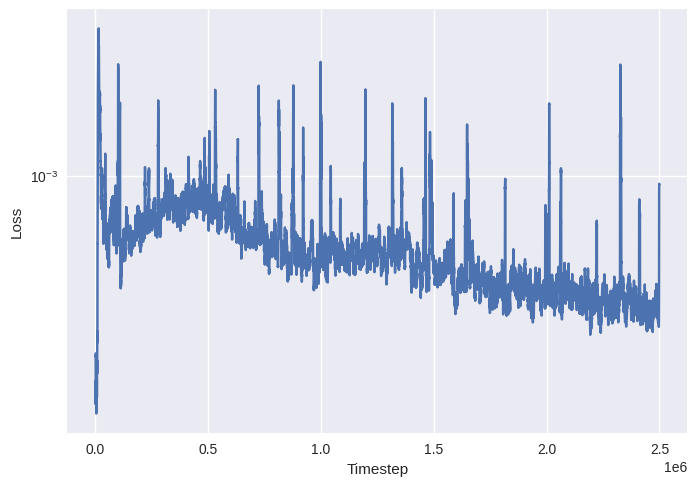
\includegraphics[scale=0.5]{../ER_20spin/eco/min_cut/network/loss.png}

%     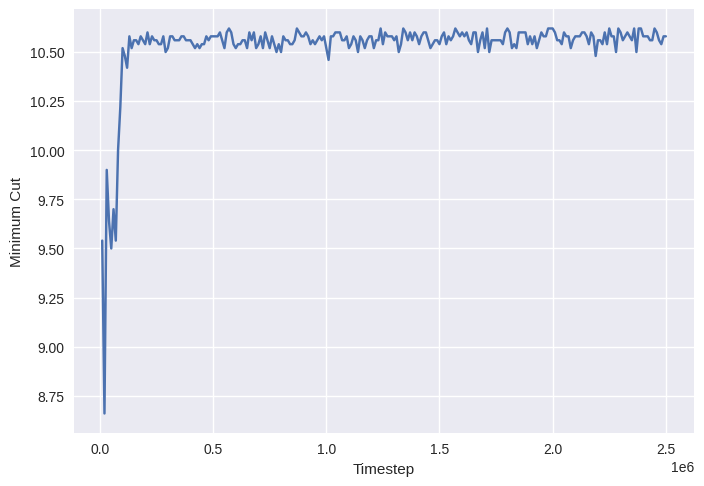
\includegraphics[scale=0.5]{../ER_20spin/eco/min_cut/network/training_curve.png}
%     \label{fig:min-cut-training}
% \end{figure}

\begin{figure}[ht]
    \caption{Training Loss and Average Solution $|V| = 20$}
    \centering
    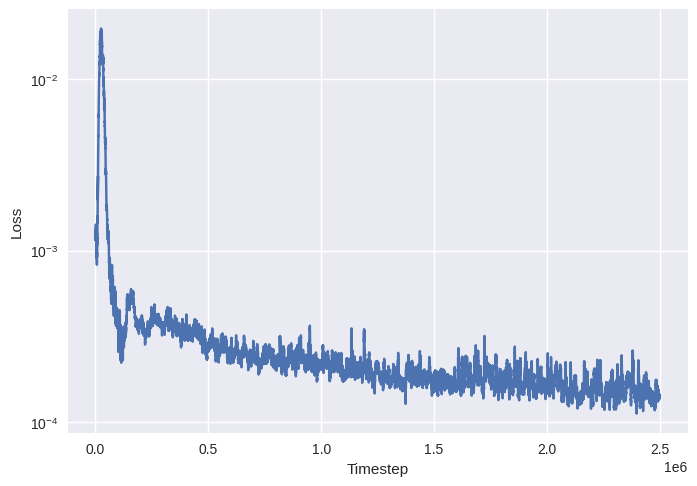
\includegraphics[scale=0.5]{../ER_20spin/eco/min_cover/network/loss.png}

    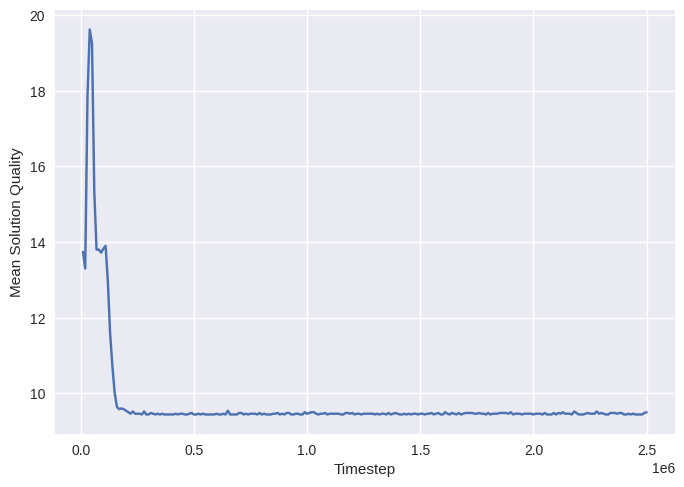
\includegraphics[scale=0.5]{../ER_20spin/eco/min_cover/network/training_curve.png}
    \label{fig:training-mvc-20}
\end{figure}



% \begin{figure}[ht]
%     \caption{Training Loss and Average Solution $|V| = 60$}
%     \centering
%     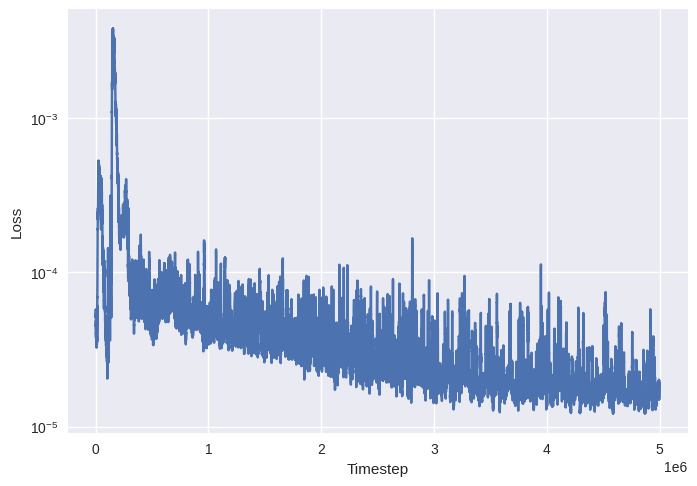
\includegraphics[scale=0.5]{../ER_60spin/eco/min_cover/network/loss.png}

%     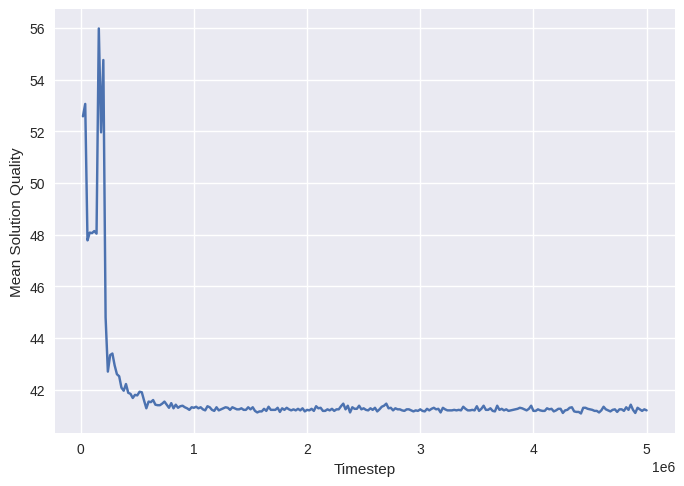
\includegraphics[scale=0.5]{../ER_60spin/eco/min_cover/network/training_curve.png}
%     \label{fig:training-mvc-60}
% \end{figure}

\begin{figure}
    \caption{Average Cover Found on Validation Graphs}
    \centering
    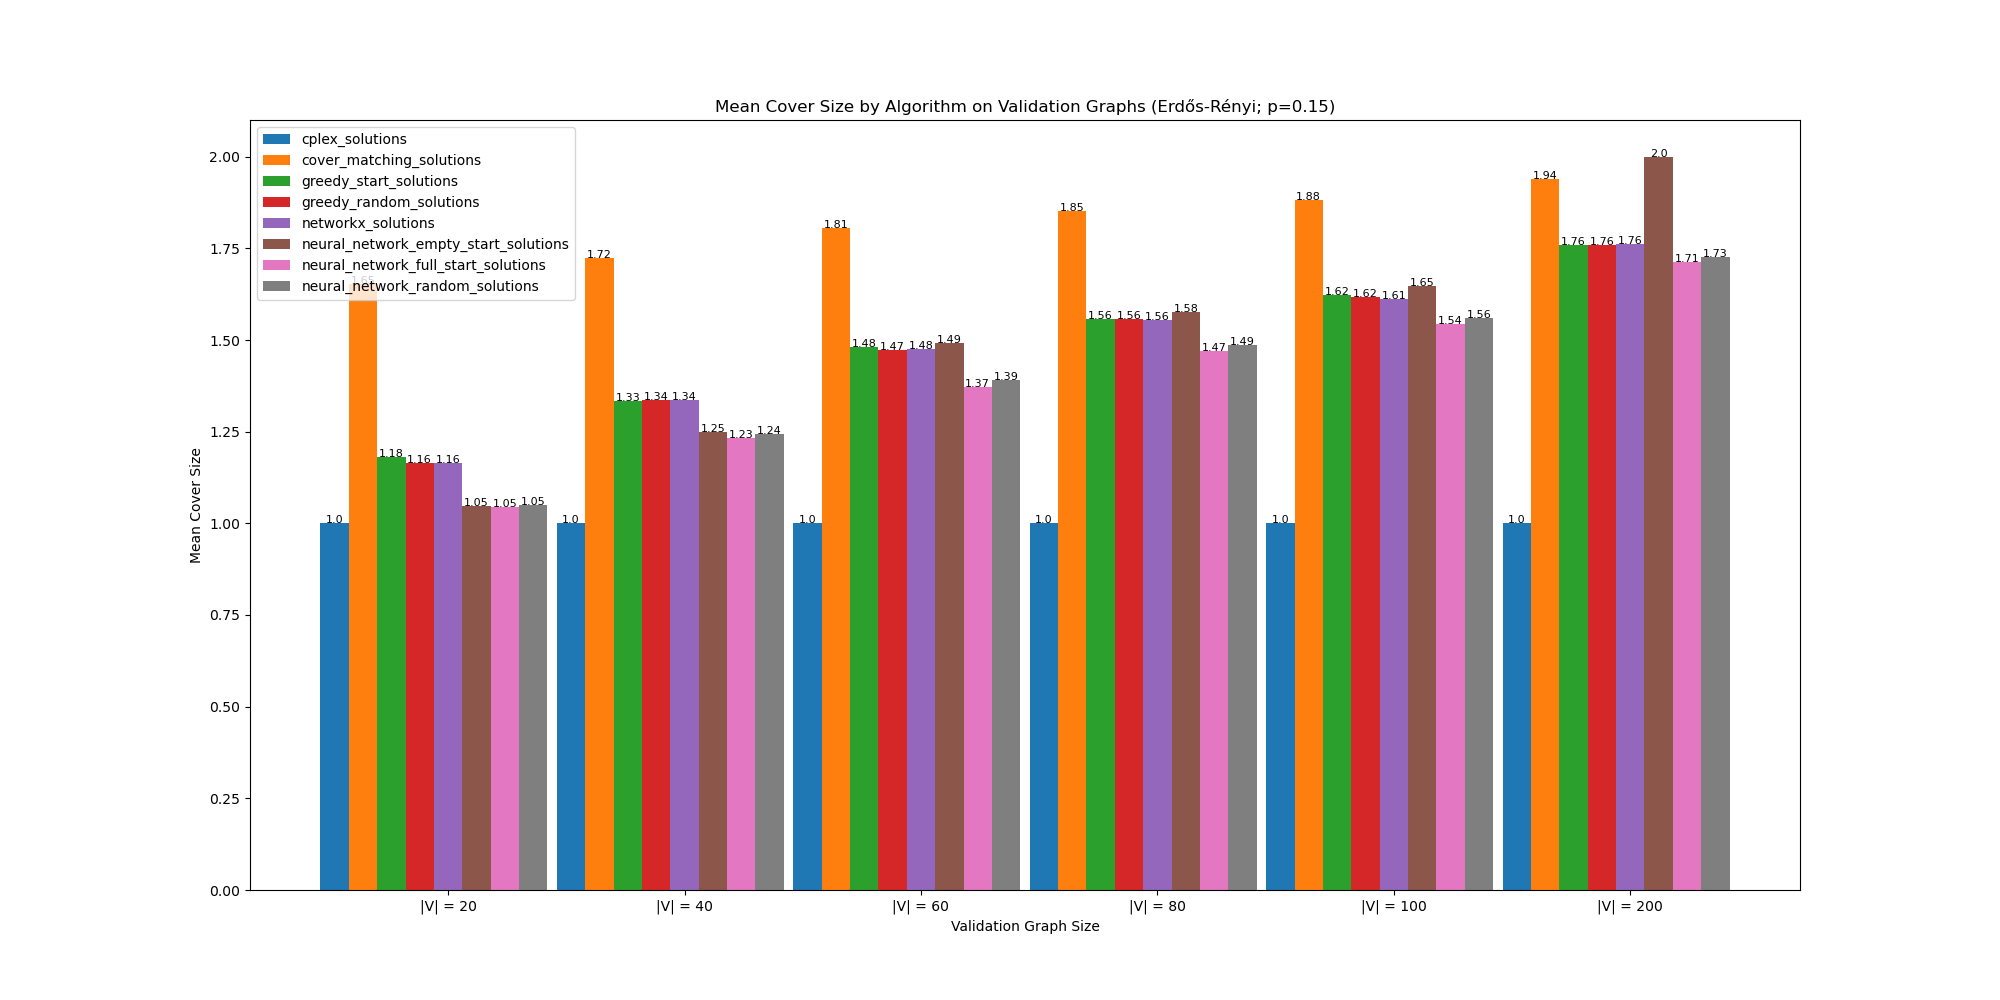
\includegraphics[scale=0.2]{../test20.png}
    \label{fig:test-20}
\end{figure}

\clearpage
\bibliography{main}
\bibliographystyle{ieeetr}


\end{document}